\chapter{Differential Equations}

Differential equations are equations involving an unknown function and
its derivatives. They play a crucial role in mathematics, physics,
engineering, economics, and other disciplines due to their ability to
describe change over time or in response to changing conditions.\index{differential equations}

\section{Ordinary Differential Equations}

An ordinary differential equation (ODE) involves a function of a
single independent variable and its derivatives. The order of an ODE
is determined by the order of the highest derivative present in the
equation. An example of a first-order ODE is:\index{ordinary 
differential equation} \index{ODEs}

\begin{equation}
\frac{dy}{dx} + y = x
\end{equation}

Here, $y$ is the function of the independent variable $x$, and 
$\frac{dy}{dx}$ represents its first derivative.

A real-world example of the application of differential equations is an 
oscillating spring (or any harmonic motion). When a spring is stretched, the 
restoring force (the force pulling or pushing it back to its neutral position) 
is proportional to the distance by which the spring has been stretched (see 
figure --- fixme image of spring at equilibrium position and displaced with 
label). Mathematically, we say that
$$\text{restoring force} = -kx$$
where $k$ is the positive spring constant (the stiffer a spring, the greater 
$k$). Recall that Newton's Second Law tells us that force is equal to mass 
times acceleration, and that acceleration is the second derivative of position. 
We can then write the differential equation:
$$m \frac{d^2x}{dt^2} = -kx$$
This is called a \textbf{second-order differential equation} because it 
involves second-order derivatives. The order of a differential equation is the 
same as the highest order of derivative in the equation. We can further 
re-write the equation to isolate the second derivative:
$$\frac{d^2x}{dt^2} = -\frac{k}{m}x$$

In everyday language, this is saying that the second derivative is proportional 
to the original function, just negative. There are two trigonometric functions 
that have this property, take a second to see if you remember and write down 
your guess. 

The sine and cosine functions both have the property $\frac{d^2x}{dt^2} \propto 
-x(t)$ (recall that $\propto$ means ``proportional to"). 

\textbf{Example}: Assuming $x(t)$ is a sine function, solve the second-order 
differential equation $\frac{d^2x}{dt^2} = \frac{-k}{m}x$.

\textbf{Solution}: Let $x(t) = \sin{Ct}$. Then $\frac{dx}{dt} = C\cos{Ct}$ and 
$\frac{d^2x}{dt^2} = -C^2\sin{t}$. This implies that $C^2 = \frac{k}{m}$ and 
$C = \pm \sqrt{\frac{k}{m}}$. So a solution to the differential equation 
$\frac{d^2x}{dt^2} = \frac{-k}{m}x$ is $x(t) = \sin{\sqrt{\frac{k}{m}}t}$. 

\subsection{Population Growth}
Another real-world application of differential equations is modeling population 
growth. Under ideal conditions (unlimited food, no predators, disease-free, 
etc.), the population of a species grows at a rate proportional to the current 
population size. We can identify 2 variables:
$$t = \text{ time (the independent variable)}$$
$$P = \text{ the number pf individuals in the population (the dependent 
variable)}$$

Then what is the rate of growth? Recall that a rate is change over time. In 
that case, the rate of growth is given by $\frac{dP}{dt}$. If the rate of 
growth is proportional to the population, then we can write a first-order 
differential equation:
$$\frac{dP}{dt} = kP$$

Where k is a proportionality constant. This is called \textbf{natural growth} 
or \textbf{logarithmic growth}\index{natural growth}\index{logarithmic growth}. 
To find a solution, we must answer the question: what function's derivative is 
a constant multiple of itself? Recall that we've seen that the derivative of 
the exponential function $e^{kt}$ is $ke^{kt}$. Setting $P(t) = Ce^{kt}$ 
(where $C$ is some constant), we see that the derivative is $\frac{dP}{dt} = 
kCe^{kt} = kP(t)$ (see figure \ref{expdiff}). You can determine C from initial 
conditions. 

\begin{figure}
\centering
    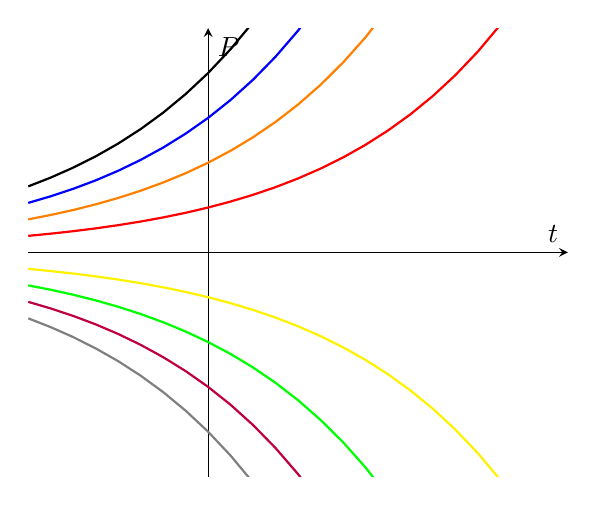
\begin{tikzpicture}
	\begin{axis}[xmin = -1, xmax = 2, ymin = -5, ymax = 5, xtick = \empty, 
	ytick = \empty, xlabel = $t$, ylabel = $P$, axis lines = center]
	\addplot[gray, thick, domain = -1:2]{-4*e^x};
        \addplot[purple, thick, domain = -1:2]{-3*e^x};
        \addplot[green, thick, domain = -1:2]{-2*e^x};
        \addplot[yellow, thick, domain = -1:2]{-1*e^x};
        \addplot[red, thick, domain = -1:2]{e^x};
        \addplot[orange, thick, domain = -1:2]{2*e^x};
        \addplot[blue, thick, domain = -1:2]{3*e^x};
        \addplot[black, thick, domain = -1:2]{4*e^x};
	\end{axis}
    \end{tikzpicture}
    \caption{Several solutions to $\frac{dP}{dt} = kP$}
    \label{expdiff}
\end{figure}


\textbf{Example}: Suppose a population of bacteria has an initial population 
of 100 bacteria. If the bacteria's growth rate is given by $\frac{dP}{dt} = 
2P$, (where $t$ is in hours) how many bacteria are present after 4 hours?

\textbf{Solution}: We have seen that the solution to $\frac{dP}{dt} = 2P$ is 
$P(t) = Ce^{2t}$. We can then use the given initial condition to find $C$:
$$P(0) = 100 = Ce^{2 \cdot 0} = C \cdot 1 = C$$
Which means that the complete solution is:
$$P(t) = 100 e^{2t}$$

To answer the question, we need to find $P(4)$:
$$P(4) = 100 e^{2 \cdot 4} = 100 e^{8} \approx 298096$$

As stated above, this model works well for populations under specific, ideal 
conditions. However, there are very few environments in which these conditions 
are met. Real animals suffer from disease, are hunted by predators, and have 
limited food supplies. Most environments have a maximum number of animals they 
can support, which ecologists call a \textbf{carrying capacity}\index{carrying 
capacity}. Let us call the carrying capacity of an environment $M$. Then the 
population growth can be modeled by the logistic differential equation: \index{
logistic differential equation}
$$\frac{dP}{dt} = kP \left( 1 - \frac{P}{M} \right)$$

This is called a \textbf{logistic differential growth model}\index{logistic 
differential growth model}. Notice that if $P$ is small, then $\frac{dP}{dt} 
\approx kP$. This makes sense: if the population is very small compared to the 
carrying capacity, the conditions are nearly ideal, and so growth should be 
nearly ideal too. On the other hand, if the population ever goes \textit{
above} the carrying capacity, the $\frac{dP}{dt} < 0$ and the population will 
decrease back below the carrying capacity (see figure \ref{logdiff}). Notice 
that if the initial population is $P_0 = M$, then $\frac{dP}{dt} = kP \left( 1 
- 1 \right) = 0$ and the population is stable at $P(t) = M$. We call this an 
\textbf{equilibrium solution}\index{equilibrium solution}. Can you logically 
find the other equilibrium solution? 

If there are no animals to begin with, then there are none to reproduce, and 
$P(t) = 0$. This is the other equilibrium solution. Notice that when the 
population is in equilibrium, then the rate of change is zero. Mathematically, 
to find equilibrium solutions, we can set $\frac{dP}{dt} = 0$ and solve for $P$. 

\begin{figure}
\centering
    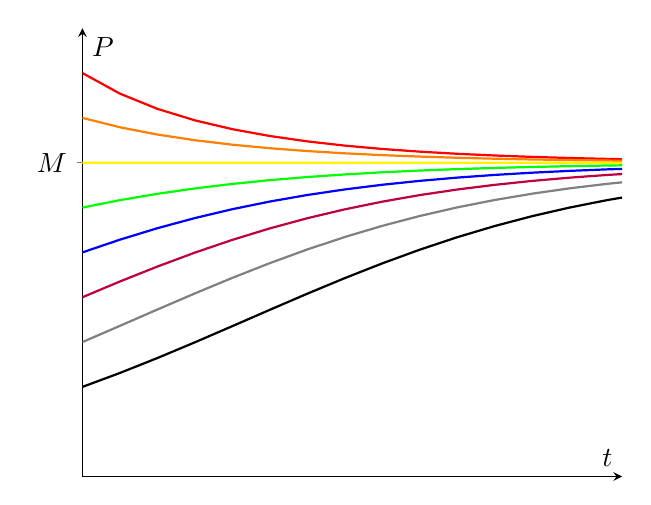
\begin{tikzpicture}
	\begin{axis}[xmin = 0, xmax = 3, ymin = 0, ymax = 10, ytick = {7}, 
	yticklabels = {$M$}, xtick = \empty, xlabel = $t$, ylabel = $P$, 
	axis lines = center]
	\addplot[gray, dashed, domain = 0:5]{7};
        \addplot[red, thick, domain = 0:5]{(9*7*e^x)/(7-9 + 9*e^x)};
        \addplot[orange, thick, domain = 0:5]{(8*7*e^x)/(7-8 + 8*e^x)};
        \addplot[yellow, thick, domain = 0:5]{(7*7*e^x)/(7-7 + 7*e^x)};
        \addplot[green, thick, domain = 0:5]{(6*7*e^x)/(7-6 + 6*e^x)};
        \addplot[blue, thick, domain = 0:5]{(5*7*e^x)/(7-5 + 5*e^x)};
        \addplot[purple, thick, domain = 0:5]{(4*7*e^x)/(7-4 + 4*e^x)};
        \addplot[gray, thick, domain = 0:5]{(3*7*e^x)/(7-3 + 3*e^x)};
        \addplot[black, thick, domain = 0:5]{(2*7*e^x)/(7-2 + 2*e^x)};
        \end{axis}
    \end{tikzpicture}
    \caption{Several solutions to $\frac{dP}{dt} = kP \left( 1 - \frac{P}{M} 
    \right)$}
    \label{logdiff}
\end{figure}

\begin{Exercise}[label = logdiff1]
A population is modeled by the differential equation $\frac{dP}{dt} = 1.2P 
\left( 1 - \frac{P}{4200} \right)$.
\begin{enumerate}
\item What is the carrying capacity of the environment?
\item For what values of $P$ is the population increasing?
\item For what values of $P$ is the population decreasing?
\item What are the equilibrium solutions?
\end{enumerate}
\end{Exercise}

\begin{Answer}[ref = logdiff1]
\begin{enumerate}
\item 4200
\item Logically, we can say that the population will increase if it is below 
the carrying capacity (that is, $P < 4200$), but we can also prove it 
mathematically: $\frac{dP}{dt} < 0 \rightarrow 1.2P \left( 1 - \frac{P}{4200} 
\right) < 0 \rightarrow P \left( 1 - \frac{P}{4200} \right) < 0$. Since we are 
talking about population, we can assume that $P > 0$ and continue: $1 - 
\frac{P}{4200} < 0 \rightarrow 1 < \frac{P}{4200} \rightarrow 4200 < P$, which 
is the result we expected. 
\item Similarly, we know the population should be decreasing when $P$ is 
greater than the carrying capacity of $4200$.
\item The equilibrium solutions can be found by setting $\frac{dP}{dt} = 0$ 
and solving. The solutions are $P(t) = 0$ and $P(t) = 4200$. 
\end{enumerate}
\end{Answer}

\begin{Exercise}[label = logdiff2]
[This problem was originally presented as a calculator-allowed, free response 
question on the 2012 AP Calculus BC exam.] Let $k$ be a positive constant. 
Which of the following is a logistic differential equation?
(a) $\frac{dy}{dt} = kt$
(b) $\frac{dy}{dt} = ky$
(c) $\frac{dy}{dt} = kt(1 - t)$
(d) $\frac{dy}{dt} = ky(1 - t)$
(e) $\frac{dy}{dt} = ky(1 - y)$
\end{Exercise}

\begin{Answer}[ref = logdiff2]
Recall that logistic differential equations are of the form $\frac{dy}{dt} = 
ky(1 - \frac{y}{m})$ where $y$ is a function and $t$ is the independent 
variable. (e) is the only logistic differential equation, with $m = 1$. 
\end{Answer}


\subsection{Separable Differential Equations}
Sometimes, differential equations can be explicitly solved. A 
first-order differential equation is separable if $\frac{dy}{dx}$ can 
be written as a function of $x$ times a function of $y$. Symbolically, 
a differential equation is separable if it takes the form 
$$\frac{dy}{dx} = g(x)f(y)$$

The equations may be solvable by separating the $x$ from the $y$ and 
integrating each side. For our generic form, we can separate the 
variables thusly if $f(y) \neq 0$: 
$$\frac{dy}{dx}\frac{1}{f(y)} = g(x)$$ 
$$\frac{1}{f(y)}dy = g(x) dx$$ \\
Integrating both sides: $$\int \frac{1}{f(y)}\,dy = \int g(x)\,dx$$.

Let's look at the example $\frac{dy}{dx} = \frac{x^2}{y}$. We can 
separate the variables by multiplying both sides by $y dx$: 
$$y dy = x^2 dx$$\\
Integrating both sides: 
$$\int y\,dy = \int x^2\,dx$$
$$\frac{1}{2}y^2 + C_1 = \frac{1}{3}x^3 + C_2$$ \\
We can combine the constants by defining $C = C_2 - C_1$. Making this 
substitution and solving for $y$, we find: 
$$y^2 = \frac{2}{3} x^3 + 2C$$ 
$$y = \sqrt{\frac{2}{3} x^3 + 2C}$$\\
Noting that $2C$ is also a constant (which we'll call $K$ for 
convenience), we find the general solution is 
$$y = \sqrt{\frac{2}{3} x^3 + K}$$ \\
A graph showing the solution for several values of $K$ is in figure 
\ref{fig:solutions}.

\begin{figure}[htbp]
\centering
	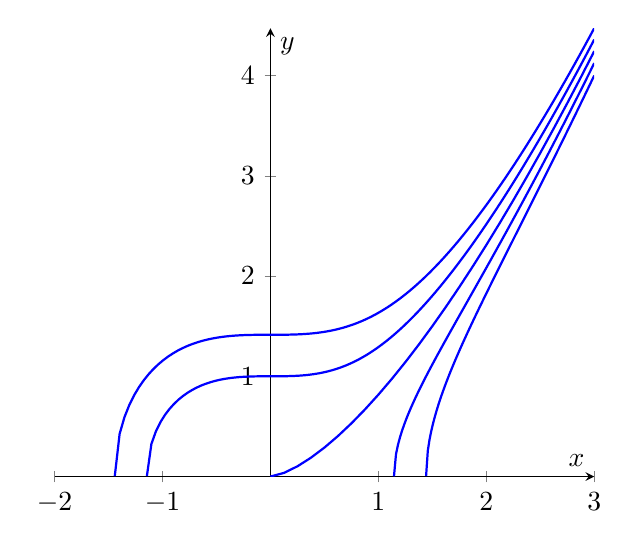
\begin{tikzpicture}
		\begin{axis}[axis lines = center, xmin = -2, xmax = 3, 
		xlabel = $x$, ylabel = $y$]
                \addplot[blue, thick, domain = 1.44226:3, samples = 100]
                {sqrt((2/3)*x^3 - 2)};
                \addplot[blue, thick, domain = 1.14472:3, samples = 100]
                {sqrt((2/3)*x^3 - 1)};
                \addplot[blue, thick, domain = 0:3]{sqrt((2/3)*x^3)};
                \addplot[blue, thick, domain = -1.14471:3, samples = 100]
                {sqrt((2/3)*x^3 + 1)};
                \addplot[blue, thick, domain = -1.44225:3, samples = 100]
                {sqrt((2/3)*x^3 + 2)};
            \end{axis}
	\end{tikzpicture}
    \caption{Several possible solutions to $\frac{dy}{dx} = 
    \frac{x^2}{y}$}
    \label{fig:solutions}
\end{figure}

It is not always possible to solve for $y$ explicitly in terms of 
$x$. The practice problem below is an example of this. 

\begin{Exercise}[label = diffeq1]
	Solve the differential equation $\frac{dy}{dx} = \frac{3x^2}{2y + \sin{y}}$. 
\end{Exercise}

\begin{Answer}[ref = diffeq1]
	$$\frac{dy}{dx} dx = \frac{3x^2}{2y + \sin{y}} dx$$
	$$(2y + \sin{y})(dy) = \frac{3x^2}{2y + \sin{y}}(2y + \sin{y})(dx)$$
	$$(2y + \sin{y})dy = (3x^2)dx$$
	$$\int 2y\,dy + \int \sin{y}\,dy = \int 3x^2\,dx$$
	$$y^2 - \cos{y} = x^3 + C$$
\end{Answer}

\begin{Exercise}[label = diffeq2]
[This problem was originally presented as a calculator-allowed, free response 
question on the 2012 AP Calculus BC exam.] The rate at which a baby bird gains 
mass is proportional to the difference between its adult mass and its current 
mass. At time $t = 0$, when the bird is first weighed, its mass is 20 grams. 
If $B(t)$ is the mass of the bird, in grams, at time $t$ days after it is 
first weighed, then $$\frac{dB}{dt} = \frac{1}{5} \left( 100 - B \right)$$
Let $y = B(t)$ be the solution to the differential equation with initial 
condition $B(0) = 20$. 
\begin{enumerate}
\item Is the bird gaining mass faster when it masses 40 grams or when it 
masses 70 grams? Explain your reasoning.
\item Find $\frac{d^2 B}{dt^2}$ in terms of $B$. Use it to explain why the 
graph of $B$ cannot resemble the graph shown below. 
\item Use separation of variables to find $y = B(t)$, the particular solution 
to the differential equation with initial condition $B(0) = 20$. 
\end{enumerate}
\begin{tikzpicture}
	\begin{axis}[xmin = 0, xmax = 15, ymin = 0, ymax = 120, xtick = \empty, 
	ytick = {20, 100}, xlabel = time (days), ylabel = weight (grams), 
	axis lines = center]
	\addplot[blue, thick, domain = 0:15]{80/(1 + 20*e^(4-x)) + 20};
	\end{axis}
\end{tikzpicture}
\end{Exercise}

\begin{Answer}[ref = diffeq2]
\begin{enumerate}
\item Since $\frac{dB}{dt}$ depends only on B, we can use the given masses to 
find the rate of growth for each mass. $\frac{dB}{dt}(40) = \frac{1}{5} \left( 
100 - 40 \right) = \frac{1}{5} \left(60 \right) = 12$ and $\frac{dB}{dt}(70) = 
\frac{1}{5} \left( 100 - 70 \right) = \frac{1}{5} \left( 30 \right) = 6$. 
Since $\frac{dB}{dt}$ is greater when $B = 40$, the baby bird is gaining mass 
faster when it has a mass of $40$ grams. 
\item $\frac{d^2 B}{dt^2} = \frac{d}{dt} \left( \frac{dB}{dt} \right) = 
\frac{d}{dt} \left[ \frac{1}{5} \left(100 - B \right) \right] = \frac{1}{5} 
\left( -\frac{dB}{dt} \right) = \frac{-1}{5} \left[\frac{1}{5} \left( 100 - B 
\right) \right] = -\frac{1}{25} \left(100 - B \right)$. For $20 < B < 100$, 
$\frac{d^2 B}{dt^2} < 0$ and the graph of $B$ should be concave down. The 
graph shown has a concave up portion, so it cannot represent $B(t)$. 
\item $\frac{dB}{dt} = \frac{1}{5} \left( 100 - B \right) \rightarrow 
\frac{dB}{100 - B} = \frac{1}{5} dt \rightarrow \int \left(100 - B \right)\,dB 
= \int \frac{1}{5}\,dt \rightarrow -\ln{100 - B} = \frac{t}{5} + C \rightarrow 
e^{\frac{-t}{5} + C} = 100 - B \rightarrow ke^{\frac{-t}{5}} = 100 - B 
\rightarrow B(t) = 100 - ke^{\frac{-t}{5}}$. Setting $B(0) = 20$ to find $k$: 
$20 = 100 - ke^{0} \rightarrow 20 = 100 - k \rightarrow k = 80$. So the 
particular solution is $B(t) = 100 - 80e^{\frac{-t}{5}}$
\end{enumerate}
\end{Answer}

\begin{Exercise}[label = popgrowth]
[This problem was originally presented as a no-calculator, multiple-choice 
question on the 2012 AP Calculus BC exam.] If $P(t)$ is the size of a 
population at time $t$, which of the following differential equations 
describes \textit{linear} growth in the size of the population?
(a) $\frac{dP}{dt} = 200$
(b) $\frac{dP}{dt} = 200t$
(c) $\frac{dP}{dt} = 100t^2$
(d) $\frac{dP}{dt} = 200P$
(e) $\frac{dP}{dt} = 100P^2$
\end{Exercise}

\begin{Answer}[ref = popgrowth]
(A). (a), (b), and (c) are all separable equations. But only the solution to A 
is linear ($P(t) = 200t + C$). (d) is logarithmic, or natural growth and (e) 
is also not linear.
\end{Answer}
\section{Partial Differential Equations}

Partial differential equations (PDEs), on the other hand, involve a
function of multiple independent variables and their partial
derivatives. An example of a PDE is the heat equation, a second-order
PDE:\index{partial differential equations} \index{PDEs}

\begin{equation}
\frac{\partial u}{\partial t} = \alpha \frac{\partial^2 u}{\partial x^2}
\end{equation}

In this equation, $u = u(x, t)$ is a function of the two independent
variables $x$ and $t$, $\frac{\partial u}{\partial t}$ is the first
partial derivative of $u$ with respect to $t$, and $\frac{\partial^2
  u}{\partial x^2}$ is the second partial derivative of $u$ with
respect to $x$.



